%\documentclass[11pt,reqno]{amsart}
%%\documentclass[a4paper,10pt]{scrartcl}
%% \oddsidemargin = 1cm
%% \textwidth = 14cm
% \topmargin = -1.0cm
%% \footskip = 3cm
%\usepackage[width=16.0cm, left=2.7cm, height=23cm, top = 2cm]{geometry}

\documentclass[11pt]{amsart}


%\usepackage[paperwidth=400.0pt,paperheight=624.0pt,margin=20.0pt]{geometry}
\usepackage[text={504pt,644pt},centering]{geometry}

\usepackage[english]{babel}
\usepackage{fancyhdr}
\usepackage[utf8]{inputenc} 
\usepackage{setspace}
\usepackage{color}
%\usepackage{refcheck}
\usepackage{amsmath, amsthm, amssymb}
\usepackage{amsfonts}
%\usepackage{showkeys}
\usepackage{enumitem}
%\usepackage[dvips]{epsfig}
\usepackage{graphicx}
\usepackage[english]{babel}
%\usepackage{enumerate}
\usepackage[hidelinks]{hyperref}
%\usepackage{showlabels}
\usepackage{cleveref}
\usepackage{soul}
\usepackage{subcaption}
\captionsetup[subfigure]{labelformat=empty}

\usepackage[export]{adjustbox}
\usepackage{wrapfig}
\usepackage{float}
\usepackage{graphicx}
\usepackage[mathscr]{euscript}
% \usepackage{biblatex}
% \addbibresource{references.bib}



% \theoremstyle{plain}
% \newtheorem{thm}{Theorem}[section]
% \newtheorem{cor}[thm]{Corollary}
% \newtheorem{lem}[thm]{Lemma}
% \newtheorem{conj}[thm]{Conjecture}
% \newtheorem{prop}[thm]{Proposition}
% \newtheorem{claim}[thm]{Claim}

% \theoremstyle{definition}
% \newtheorem{defi}[thm]{Definition}

% \theoremstyle{remark}
% \newtheorem{rem}[thm]{Remark}


% \numberwithin{equation}{section}
% \renewcommand{\theequation}{\thesection.\arabic{equation}}
% \renewcommand{\thefigure}{\thesection.\arabic{figure}}

\pagestyle{fancy}
\fancyhf{}
\fancyhead[RE,RO]{Joaquin Garcia-Suarez}
\fancyhead[LE,LO]{\it{Teaching Statement }}
\headsep = 0.75cm

%\cfoot{Page \thepage\ of 2}


\fancypagestyle{firststyle}
{
\fancyhf{}
\fancyhead[RE,RO]{Joaquin Garcia-Suarez}
\fancyhead[LE,LO]{\it{Teaching Statement }}
\headsep = 0.75cm
%\cfoot{\thepage\ of 2}
}


\newcommand{\X}{\mathfrak{X}}
\newcommand{\de}{\partial}
\newcommand{\on}{\overline{\nabla}}
\newcommand{\fls}{(-\Delta)^s}
\newcommand{\R}{\mathbb{R}}
\newcommand{\C}{\mathbb{C}}
\newcommand{\Z}{\mathbb{Z}}
\newcommand{\N}{\mathbb{N}}
\newcommand{\So}{\mathcal{S}}
\newcommand{\Lo}{\mathcal{L}}
\newcommand{\K}{\mathcal{K}}
\newcommand{\F}{\mathcal{F}}
\newcommand{\eps}{\varepsilon}

\newcommand{\average}{{\mathchoice {\kern1ex\vcenter{\hrule height.4pt
width 6pt depth0pt} \kern-9.7pt} {\kern1ex\vcenter{\hrule
height.4pt width 4.3pt depth0pt} \kern-7pt} {} {} }}
\newcommand{\ave}{\average\int}
\def\R{\mathbb{R}}

% \usepackage{titlesec}
% \titleformat*{\section}{\fontsize{0}{0}\selectfont}
%\titleformat*{\subsection}{\fontsize{13}{17}\selectfont}


% \date{}
% \author{}

\begin{document}

% \onehalfspacing


% \begin{center}
% \vspace{0.5cm}
% {\LARGE  
% %SNSF Ambizione Call 2022 ---
% J. Garcia-Suarez's Teaching Statement}
% % \\[0.2cm]
% % {\large\bf }
% \end{center}

% \vspace{-0.1cm}
% %\section{Summary}
% \vspace{-0.0cm}
% \thispagestyle{empty}
\thispagestyle{firststyle}


%\subsection*{Teaching Overview} 
\subsection*{Overview} My teaching style resembles my research style: I weave the \textbf{technological, physical and mathematical} strands to introduce problems in all their complexity. 
%
I cherish science outreach, and, to me, the first place to do so is the classroom. Teaching and mentoring help deepen my understanding of concepts, and thus they \textbf{foster my research}. I can proudly say that a publication of mine \cite{Fundamentalmode}
grew from a question posed by an outstanding student: \textit{ what does ``resonance” really mean?} I encourage interactions grounded in mutual respect and a shared passion for science, \textbf{supporting students from diverse backgrounds} by ensuring their perspectives help shape how we approach the material.
\vspace{-0.1cm}

\begin{wrapfigure}{l}{.5\textwidth}
    \begin{minipage}{\linewidth}
    % 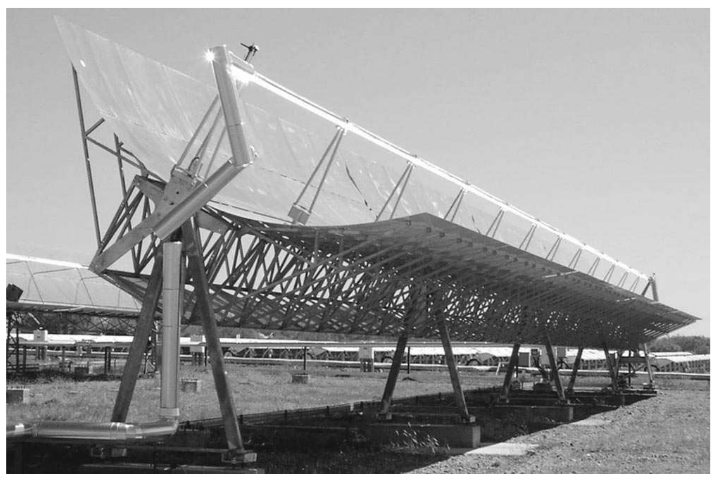
\includegraphics[width=\linewidth]{figures/parabolic_trough_pic.png}
    % \subcaption{(a) Parabolic trough solar collector (Image credit: Plataforma Solar Almeria \cite{solar})}
    % \label{fig:5a} \par\vfill
    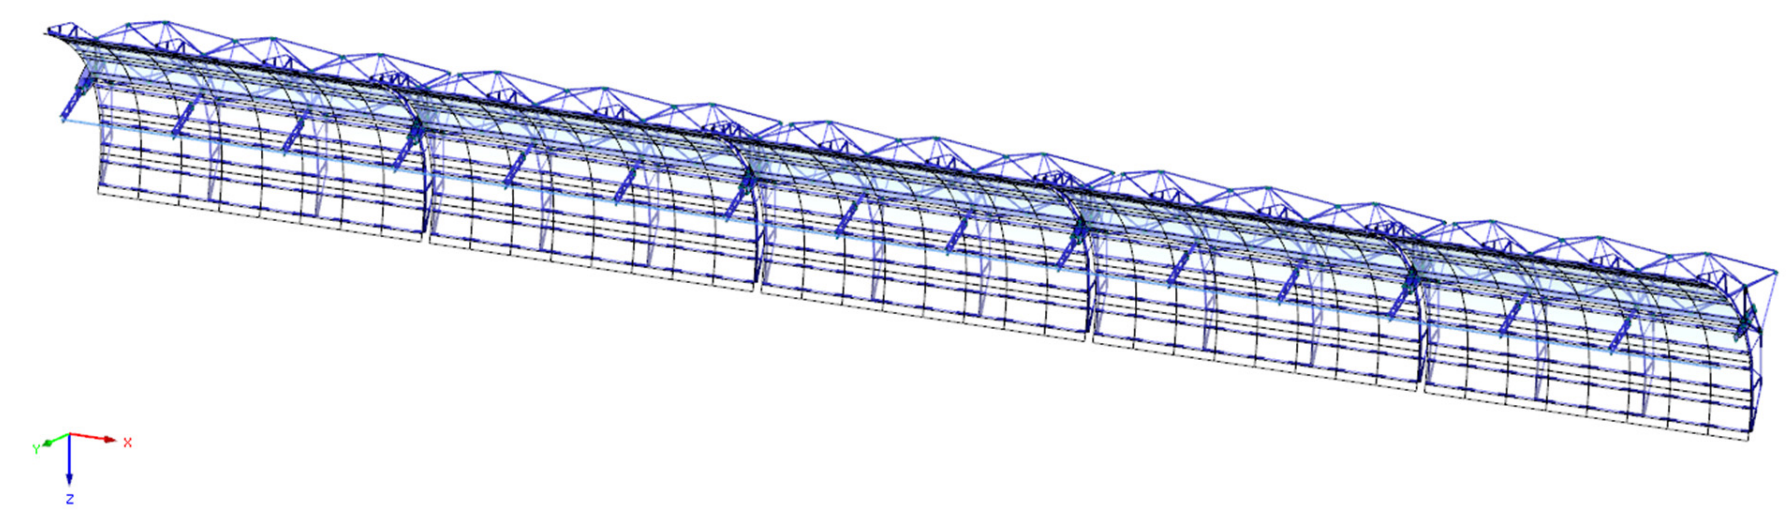
\includegraphics[width=\linewidth]{figures/collector_fem.PNG}
    \subcaption{(a) FEM model of a five-module parabolic solar collector}
    \label{fig:5a}
    \vspace{0.2cm}
    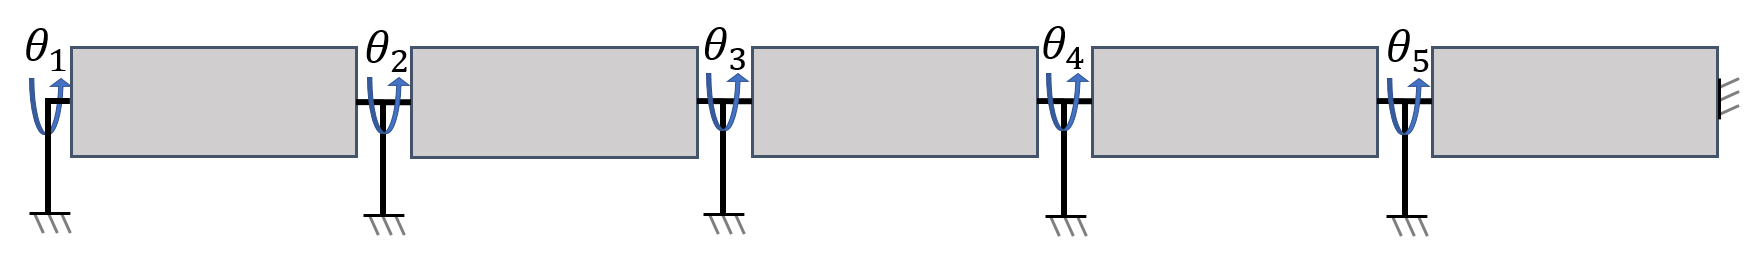
\includegraphics[width=\linewidth]{figures/collector.png}
    \subcaption{(b) Scheme highlighting torsion degrees of freedom}
    \label{fig:5c}
    \vspace{0.5cm}
    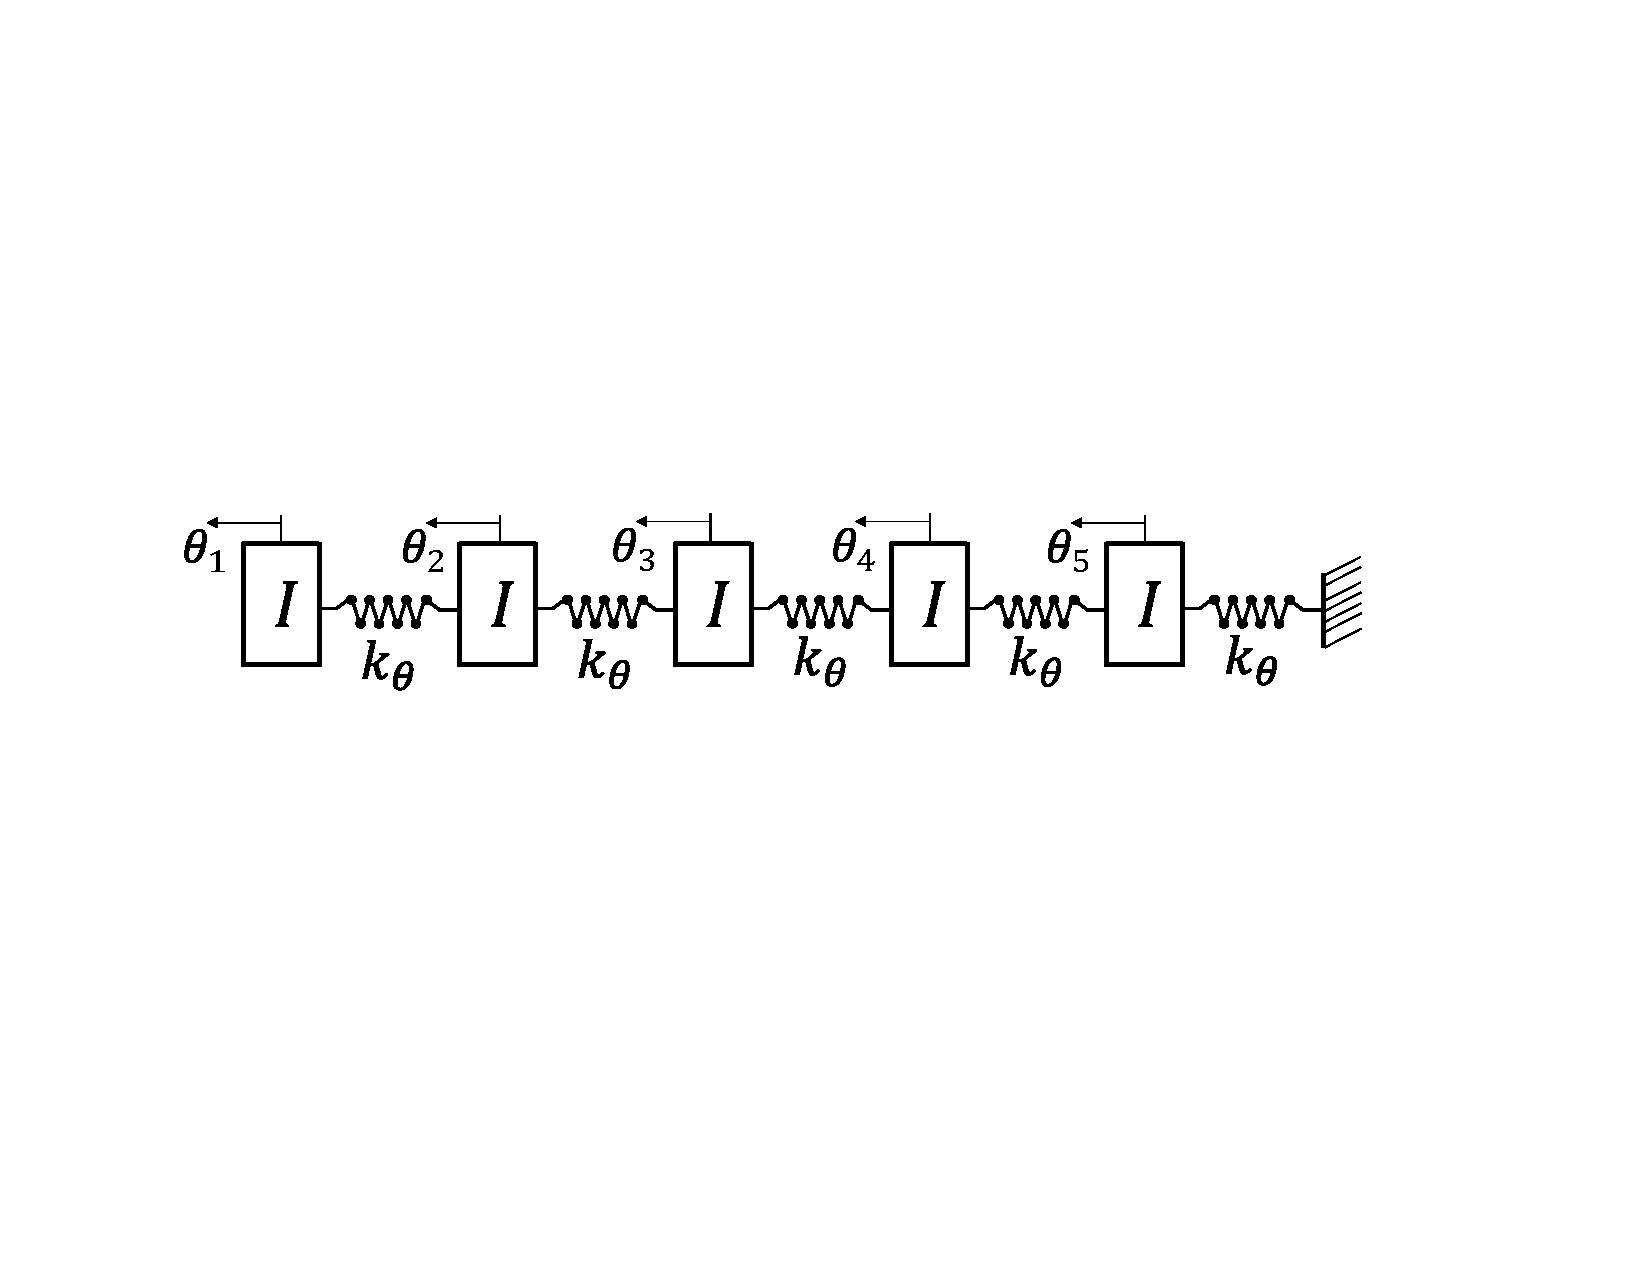
\includegraphics[width=\linewidth]{figures/model_hw.pdf}
    \subcaption{(c) Five-dof lumped torsional vibration model}
    \label{fig:5b}
\end{minipage}
\vspace{-2mm}
\caption{Solar collectors as a dynamic torsional system excited by wind loads (angle $\theta$, polar moment of inertia $I$, and module torsional spring $k_{\theta}$).}\label{fig:DDCM}
\end{wrapfigure}

\subsection*{Teaching and mentoring experience} I acted as \textbf{teaching assistant} (TA) during the academic years 2017-18, 18-19 and 19-20, in the context of AM/CE 151a \textbf{Dynamics and Vibrations}.
%, which covered an introduction to structural dynamics. 
Prof. Asimaki entrusted me with daily operations (grading, office hours, recitations and exercise sessions) 
% , maintaining the Moodle page, 
and occasional lectures. 
%
My enthusiasm was rewarded in the feedback reports (I was recognized with the campus-wide ``\textbf{best TA distinction}'' in the fall term 17-18). 
% This class also gave me the opportunity to deliver online lectures (a total of three lectures). 
%
During the spring semester 21-22, I collaborated with Prof. Molinari in the context of CIVIL-422 \textbf{Advanced Continuum Mechanics} (an introduction to finite-kinematics elasticity and to constitutive modeling) preparing lectures, holding office hours and occasionally teaching when he was on travel. 
%
Again, during the spring semester 23-24, I aided him and Prof. Lecampion with a new class of similar scope, CIVIL-425 \textbf{Continuum Mechanics and Applications}. 
% 
I served as the primary instructor in the spring semester 24-25, receiving positive reviews (see attached CV). 
%
At EPFL, I have supervised ten semester projects (bachelor and master) and two master theses. 
%
My first PhD student, Mr. Gaëtan Cortes, passed his candidacy exam in October 2025. 

\vspace{-0.1cm}

\subsection*{Teaching methods} 
%
I lecture using the board and emphasizing \textbf{threshold concepts} \cite{threshold} openly, thus trying to ensure that the foundational concepts are assimilated before building upon.  
%
% Continuous reflection, evaluation and feedback is encouraged, for instance by means of weekly homework sets. 
%
This strategy leads to 
a continuous expansion of students’ \textbf{zone of proximal development} \cite{PD}; the goal is that they can continue delving in the subject as independent learners.  
%
%Having said this, I would be interested in exploring modern pedagogical techniques (e.g., ``peer instruction'').
%
% As to \textbf{design of exercises}, 
I look for inspiration in my \textbf{own experience}. 
% (i.e., those cases whose insights and intricacies I understand deeply and can convey most effectively); 
%
E.g., 
Figure 1 shows a modular trough collector — a system I once designed in \textbf{industry} — known to display torsional vibrational modes when excited by wind, which made for an exam exercise. 




\subsection*{New classes}
At the \textbf{graduate level}, I would like to eventually prepare two new one-semester classes.  
%
``\textbf{Fluid-Solid Interactions at Low Reynolds Numbers}'' would provide a broad introduction to problems in which solid deformation and thin fluid layers are strongly coupled; it would cover both the continuum mechanics fundamentals together with selected applications, e.g., elastohydrodynamic lubrication \cite{EHL} and haptics \cite{haptics}.  
%
``\textbf{Group Theory for Engineers}'' would introduce basic notions of group theory \cite{Artin}
(group axioms, isomorphisms, symmetries) 
while illustrating these concepts with examples, e.g., 3D space rotations using $SO(3)$ and transfer matrices for wave propagation as elements of $SL_2 (\mathbb{R})$ \cite{JMPS}. 

\newpage

\thispagestyle{plain}
\pagenumbering{gobble}
%\printbibliography
%\bibliography{references}
%\bibliographystyle{plain}
% \bibliography{references}
% \bibliographystyle{acm}

% \renewcommand\refname{References}  


\section*{References}

\begingroup
\renewcommand{\section}[2]{}%
\begin{thebibliography}{99}

     \bibitem[1]{Fundamentalmode}
	\newblock \textbf{Garcia-Suarez, J.}, Asimaki, D. (2020)
	\newblock ``On the fundamental resonance mode of inhomogeneous soil deposits''.
	\newblock \emph{Soil Dynamics and Earthquake Engineering}. 

    % \bibitem[2]{research-led}
    % \newblock Deakin, M. (2006)
    % \newblock ``Research-led teaching: a review of two initiatives in valuing the link between teaching and research''.
    % \newblock \emph{Journal for Education in the Built Environment}.

    \bibitem[2]{threshold}
    \newblock Meyer, J., Land, R. (2003)
    \newblock ``Threshold concepts and troublesome knowledge: linkages to ways of thinking and practising within the disciplines''.

    \bibitem[3]{PD}
    \newblock Fila, N., Fernandez, T., Purzer, S., Bohlin, A. (2016)
    \newblock \emph{Innovation and the zone of proximal development in engineering education}.
    \newblock In: 2016 ASEE Annual Conference \& Exposition.

    \bibitem[4]{EHL} 
    \newblock Dowson, D., and Higginson, G. R. (2014)
    \newblock \textit{Elasto-Hydrodynamic Lubrication}. 
    \newblock Publisher: Pergamon. 
    % Editor: D. W. Hopkins. 
    % eBook ISBN: 9781483181899

    \bibitem[5]{haptics}
    \newblock Wiertlewski, M., Fenton Friesen, R., and Colgate, J. E. (2016)
    \newblock ``Partial squeeze film levitation modulates fingertip friction'',
    \newblock \textit{Proceedings of the National Academy of Sciences}

    \bibitem[6]{Artin}
	\newblock Artin, M. (2011)
	\newblock \emph{Algebra (2nd edition)}.
	\newblock Publisher: Prentice Hall.
		
    \bibitem[7]{JMPS}
    \newblock \textbf{Garcia-Suarez, J.} (2022)
    \newblock ``Harmonic decomposition of the trace of 1D transfer matrices in layered media'', 
    \newblock \emph{Journal of the Mechanics and Physics of Solids}.


    % \bibitem[7]{PINNs}
    % \newblock Raissi, M., Perdikaris, P., Karniadakis, G. (2019)
    % \newblock ``Physics-informed neural networks: A deep learning framework for solving forward and inverse problems involving nonlinear partial differential equations''.
    % \newblock \emph{Journal of Computational Physics}.
    
    % \bibitem[7]{Trent}
    % \newblock Kirchdoerfer, T., Ortiz, M. (2016)
    % \newblock ``Data-driven computational mechanics''.
    % \newblock \emph{Computer Methods in Applied Mechanics and Engineering}.
	
% 	\vspace{0mm}
 %    \bibitem[8]{Mohr}
 %    \newblock Bonatti, C., Mohr, D. (2021)
 %    \newblock ``One for all: universal material model based on minimal state-space neural networks''.
 %    \newblock \emph{Science Advances}. 

 %     \bibitem[9]{Liu}
	% \newblock Liu, B., Ortiz, M., Cirak, F. (2024)
	% \newblock ``Towards quantum computational mechanics''.
	% \newblock \emph{Computer Methods in Applied Mechanics and Engineering}.
	
	

	
	

		

%	
%	
%*****
%\vspace{0mm}
%\bibitem[FS20]{FS19}
%	\newblock X. Fern\'andez-Real, J. Serra,
%	\newblock \emph{Regularity of minimal surfaces with lower dimensional obstacles},
%	\newblock J. Reine Angew. Math. 767 (2020), 37-75.
\end{thebibliography}




\end{document}
